\documentclass[preprint,3p,12pt]{elsarticle}
\usepackage{amsmath}
\usepackage{color}
\usepackage{xcolor}
\usepackage{amsmath}
\usepackage{tikz}
\usetikzlibrary{arrows.meta, positioning, calc}
\usepackage{pgfplots}

\newcommand{\qair}{q}

\begin{document}

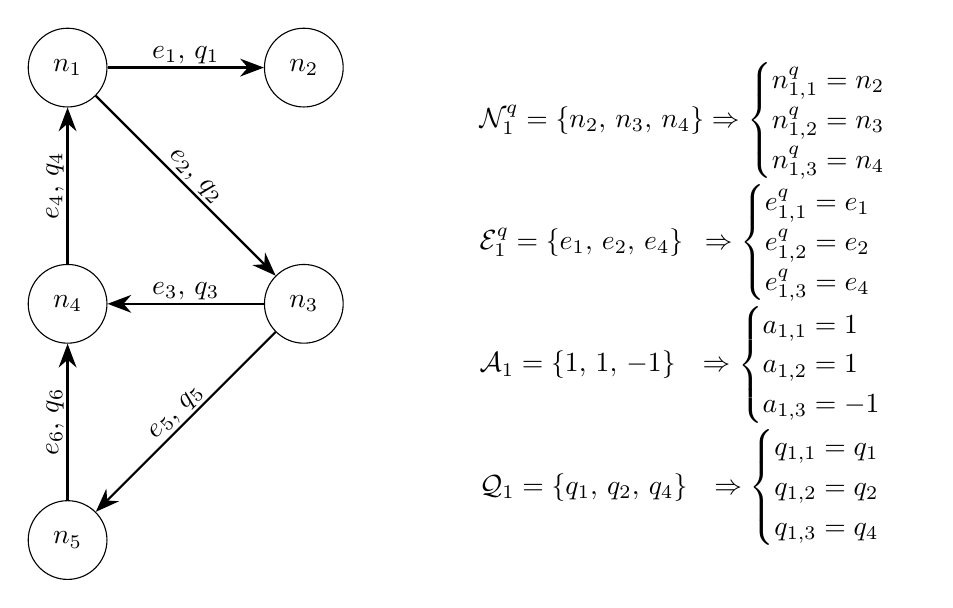
\begin{tikzpicture}[
    node/.style={draw, circle, minimum size=1.cm},
    edgelabel/.style={midway, fill=none, inner sep=1pt, sloped},
    every edge/.style={draw, -{Stealth}, thick}
]
\def \elen{3}
% Nodes
\node[node] (node1)  at (0,0)   {$n_{1}$};
\node[node] (node2) at (\elen,0) {$n_{2}$};
\node[node] (node3) at (\elen,-\elen) {$n_{3}$};
\node[node] (node4) at (0,-\elen) {$n_{4}$};
\node[node] (node5) at (0,-2*\elen) {$n_{5}$};
% Edges with rotated labels (sloped)
\draw[-{Stealth[scale=1.3]}, line width=0.8pt] (node1)  -- node[edgelabel, above] {$e_1,\,\qair_1$} (node2);

\draw[-{Stealth[scale=1.3]}, line width=0.8pt] (node1) -- node[edgelabel, above] {$e_2,\,\qair_2$} (node3);

\draw[-{Stealth[scale=1.3]}, line width=0.8pt] (node3) -- node[edgelabel, above] {$e_3,\,\qair_3$} (node4);

\draw[-{Stealth[scale=1.3]}, line width=0.8pt] (node4) -- node[edgelabel, above] {$e_4,\,\qair_4$} (node1);

\draw[-{Stealth[scale=1.3]}, line width=0.8pt] (node3) -- node[edgelabel, above] {$e_5,\,\qair_5$} (node5);

\draw[-{Stealth[scale=1.3]}, line width=0.8pt] (node5) -- node[edgelabel, above] {$e_6,\,\qair_6$} (node4);

\node[align=left] at (\elen+5,-\elen) {$\mathcal{N}^q_1=\{n_2,\,n_3,\,n_4\}\Rightarrow\begin{cases}n_{1,1}^q=n_2\\n_{1,2}^q=n_3\\ n_{1,3}^q = n_4\end{cases}$\\ $\mathcal{E}^q_1=\{e_1,\,e_2,\,e_4\}\hspace{0.5em}\Rightarrow\begin{cases}e_{1,1}^q=e_1\\e_{1,2}^q=e_2\\ e_{1,3}^q = e_4\end{cases} $\\ $\mathcal{A}_1=\{1,\,1,\,-1\}\hspace{0.7em}\Rightarrow \begin{cases} a_{1,1}=1\\ a_{1,2}=1\\ a_{1,3}=-1 \end{cases}$\\ $\mathcal{Q}_1=\{q_1,\,q_2,\,q_4\}\hspace{0.7em}\Rightarrow \begin{cases} q_{1,1}=q_1\\ q_{1,2}=q_2\\ q_{1,3}=q_4 \end{cases}$};
\end{tikzpicture}

\end{document}